\chapter{Big-O}
For a job there may be available many algorithms.
One may be better in that it is faster in the long run
(or consumes less of some other resource, such as space).
That is, an algorithm's time taken 
is a function whose input is the size of the input.
Generally, larger input takes more time.
We will give the mathematical tools to describe 
the growth of these functions.

\section{Definition}
We will not need to analyze the growth of these functions precisely.
Instead, we will make some simplyfing assumptions.
We will not need to worry about constant factors, for instance.
Nor will we need to worry about initial intervals.

\subsection{Motivation}
To determine if a number~$n\in\N$ is prime, two of the methods available are 
the sieve and the Fermat test.
To find if $n$ is prime
the sieve takes about $\sqrt{n}$ many ticks, while 
the Fermat test takes about $10\cdot \lg(n)$ ticks.\footnote{Recall that $\lg(n)=\log_2(n)$ is defined by: start with~$n$ and then find
the power of $2$
that produces it.
So, if $n=8$ then $\lg(n)=3$.
If $n=10$ then $\lg(n)\approx 3.32$.}

Comparing the two, at first the sieve seems best.
For instance, for $x=1000$ the values are $\sqrt{1000}\approx 31.62$
and $10\cdot\lg(1000)\approx 99.66$.
\begin{center}
  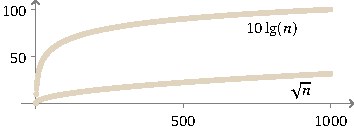
\includegraphics{complexity/asy/bigo/bigo00.pdf}
\end{center}
However,
in the long run the values of $\sqrt{x}$ are much larger than
the values of $10\lg(x)$.
For instance, $\sqrt{1\,000\,000}=1\,000$ while
$10\lg(1\,000\,000)\approx 199.32$.
\begin{center}
  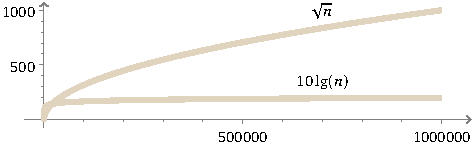
\includegraphics{complexity/asy/bigo/bigo01.pdf}
\end{center}

\margingraphic[l]{0.20\textwidth}{complexity/knuth.jpg}{\label{fig:knuth}\href{https://en.wikipedia.org/wiki/Donald_Knuth}{Donald Knuth b~1938 A pioneer of algorithm analysis}}
We can analyze the behavior of algorithms at length, finding exact algebraic expressions for how long they take, or how much memory, or how many disk reads, etc.
But for our purposes, 
we are usually interested in the long-term behavior of the function
on the large scale, as typified by the above graph,
We will therefore discount any initial chopping and changing.
Consonant with that, note that the factor of $10$ in $10\lg(x)$ is
unimportant; what matters is that a logarithm function~$10\ln(x)$ grows slower
than does a power function~$x^{1/2}$.
We will also take the view, in the definition below, that 
in choosing between two long term behaviors like the ones shown above,
we should discount constant factors.

\begin{example}
  
\end{example}




This definition reflects those considerations.

\begin{definition}
Let $\fcn{f,g}{\N}{\N}$.
Then \definend{$f$ is $\bigOh(g)$, written $f=\bigOh(g)$},
read ``$f$ is big-oh of $g$,''
when there are constants $N,C\in\N$ such that 
whenever $n>N$ then $f(n)<C\cdot g(n)$. 
\end{definition}

Think of `$f$ is $\bigOh(g)$' as meaning that
$f$'s growth rate is less than or equal to $g$'s rate.

\begin{remark}
The `$=$' notation is awkward but standard.
(sometimes written $f\in\bigOh(g)$), % or $f(n)=bigOh(g(n))$,
\end{remark}





\chapter{Computational resources}


\section{\textbf{NP}}
These two  
computational problems seem similar.

\begin{example}
Formally, a mathematical proof as a sequence of statements,
$\sigma_0$, $\sigma_1$, \ldots, $\sigma_k$,
where the final statement is the conclusion. 
Each statement either is itself an axiom or
else follows from the statements before it
by an application
of one of the agreed-upon derivation rules.
From experience we know that finding the proof of a desired  
conclusion can be very hard; often it seems to take a leap of insight.
Trying to brute-force it by taking all combinations of 
all the axioms and all the derivation rules would be very slow.
In contrast, if we were given the 
sequence of statements along with a description
of each step's rules, and asked only to check the 
sequence for correctness,
then that would be easy and quick.
\end{example}

\begin{example}
Consider a complicated propositional logic expression, say
$(\neg(P_1\vee (P_2\wedge P_3)\rightarrow \neg P_4)\leftrightarrow (P_2\rightarrow P_3)\rightarrow (P_1\wedge \neg P_4)$.
We want to find whether it is \definend{satisfiable}, 
whether there is any assignment of 
truth values $\true$ or~$\false$ to the 
variables $P_1,\idots, P_4$ that makes the statement
as a whole have the value $\true$.
We can imagine trying to answer by reasoning
in some way as, 
``Well, the formula has an if and only if arrow so I can see that
it boils down to \ldots''
but an algorithm that unfailingly finds the solution that way is not evident.
Alternatively, 
you could go through the possible assignments
$\seq{\false, \false, \false, \false}$, 
then $\seq{\false, \false, \false, \true}$, etc., 
until one causes the statement to yield $\true$, if one ever does.
However, if instead you were given an answer, an assignment to the variables,
and only asked to verify that it solves the problem, then you 
could do that quickly.
\end{example}

These seem alike in that, putting aside brute force,
we feel that for each finding an answer is hard and somehow involves creativity.
But if we are simply handed a solution then verifying that it is right 
calls only for a dull calculation.

That is, there are problems where finding an answer is quick and easy.
The two problems above seem different\Dash they \emph{feel} hard to solve, 
although
they have the property that once an answer is given then it is easy
to check.
Despite this very strong feeling, though, we are today unable
to prove that they are of different hardnesses.
This question of whether we can tell the two apart
is certainly the sexiest one in Computing today.
One reason it is attractive is that many pressing problems
have been shown to be like the proof-generating or satisfiability questions:
they don't appear to be solvable efficiently
their solutions can be verified quickly.
however, we cannot today prove that  
that is the case.  




\section{Complexity classes}
 
\begin{definition}[the complexity class $\compclass{NP}$]
A language $\lang{L}$ is a member of 
$\compclass{NP}$ if there is a polynomial $\map{p}{\N}{\N}$ and a
polynomial time Turing machine $\TM$, the \definend{verifier}
for $\lang{L}$, such that 
\begin{equation*}
  \forall \sigma\in\strings 
  \big[ \sigma\in\lang{L} 
     \,\Longleftrightarrow\, 
     \exists w\in \set{0,1}^{p(|\sigma|)}(\TM(\seq{\sigma,w})=1)  \big]
\end{equation*}
($w$ is the \definend{witness} or \definend{certificate} for $\sigma$).
\end{definition}

Note that the witness is restricted in length so that the verifier,
which as a Turing machine reads one bit at a time, can 
read it through in polynomial time.
Note also that we can take the polynomial~$p$ to be trivial $p(i)=0$
to get that $\compclass{P}\subseteq\compclass{NP}$.

\begin{exercises}
\begin{exercise}
In the definition of 
the complexity class $\compclass{NP}$, 
there is a different witness~$w$ for each~$\sigma$.
What if there is a single witness that works for all~$\sigma$?
\end{exercise}
\end{exercises}

% Use this as an example
% https://en.wikipedia.org/wiki/Belphegor%27s_prime

% Two algorithms, one is fast and one is slow
% http://blog.plover.com/2017/02/21/#anagram-scoring





% ===============================================================

\extra{Sudoku is $\compclass{NP}$ complete}

